\newcommand{\trig}{trigonometrijskih funkcija}
Osnovne trigonometrijske funkcije su sinus, kosinus, tanges i kotangens.
Funkcija kosinus ekvivalenta je funkciji sinus uz fazni pomak of \(\frac{\pi}{2}\), a kotangens je tangens na potenciju minus jedan.
Iz tog razloga ću se usredotočiti na funkcije sinus i tanges.
Sinus nalazimo u obliku:
\[f(x) = sin(x),\]
a tangens:
\[f(x) = tg(x) = \frac{sin(x)}{cos(x)},\; x \notin \{k\pi, k \in \mathbb{Z}\}.\]
\subsubsection{Domena i kodomena \trig}
    Domena funkcije sinus je skup realnih brojeva, a kodomena mu je otvoren skup of jedan do minus jedan.
    Domena funlcije tangens je skup realnih brojeva osim višekratnika broja \(\pi\), a kodomena mu je skup realnih brojeva.
    Koeficijent isprek trigonometrijske funkcije zovemo \emph{amplituda}, ona nam određuje krajnje vrijednosti funkcije.
    Parametar koji dodajemo argumentu kod trigonometrijskih funkcija zovemo \emph{fazni pomak}.
    Množimo li argument nekim Koeficijentom, povećat ćemo, ili smanjit period funkcije.

\subsubsection{Graf \trig}
    Graf funkcija sinus i kosinus zovemo sinusoida.
    \begin{figure}[ht]
        \centering
        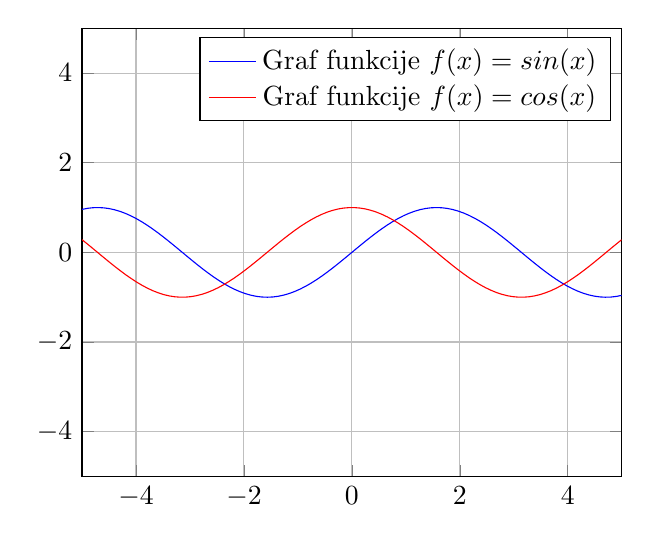
\begin{tikzpicture}
            \begin{axis}[
                grid=major,
                ymin=-5,
                ymax=5,
                xmin=-5,
                xmax=5,
            ]
                \addplot[
                    color = blue,
                    samples = 100,
                ]{sin(deg(x))};
                \addlegendentry{Graf funkcije  \(f(x) = sin(x)\)}
                \addplot[
                    color = red,
                    samples = 100,
                ]{cos(deg(x))};
                \addlegendentry{Graf funkcije  \(f(x) = cos(x)\)}
            \end{axis}
        \end{tikzpicture}
        \caption{Grafovi funkcija sinus i kosinus}
        \label{fig:template}
    \end{figure}
    \\
    \begin{figure}[ht]
        \centering
        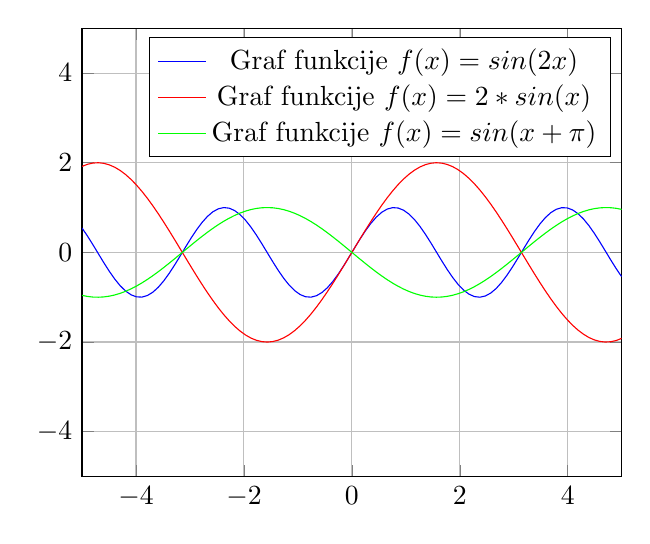
\begin{tikzpicture}
            \begin{axis}[
                grid=major,
                ymin=-5,
                ymax=5,
                xmin=-5,
                xmax=5,
            ]
                \addplot[
                    color = blue,
                    samples = 100,
                ]{sin(deg(2 * x))};
                \addlegendentry{Graf funkcije  \(f(x) = sin(2x)\)}
                \addplot[
                    color = red,
                    samples = 100,
                ]{2 * sin(deg(x))};
                \addlegendentry{Graf funkcije  \(f(x) = 2 * sin(x)\)}
                \addplot[
                    color = green,
                    samples = 100,
                ]{sin(deg(x + 3.1415))};
                \addlegendentry{Graf funkcije  \(f(x) = sin(x + \pi)\)}
            \end{axis}
        \end{tikzpicture}
        \caption{Grafovi funkcije sinus s raznim parametrima}
        \label{fig:template}
    \end{figure}
    \\
    \begin{figure}
        \centering
        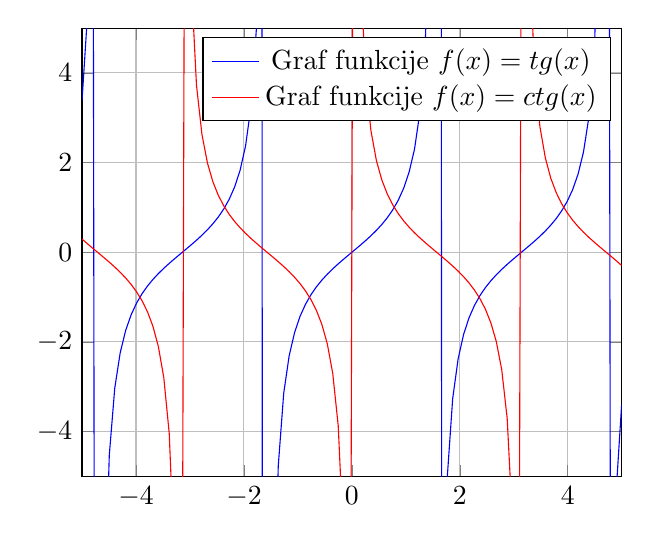
\begin{tikzpicture}
            \begin{axis}[
                grid=major,
                ymin=-5,
                ymax=5,
                xmin=-5,
                xmax=5,
            ]
                \addplot[
                    color = blue,
                    samples = 100,
                ]{tan(deg(x))};
                \addlegendentry{Graf funkcije  \(f(x) = tg(x)\)}
                \addplot[
                    color = red,
                    samples = 100,
                ]{cot(deg(x))};
                \addlegendentry{Graf funkcije  \(f(x) = ctg(x)\)}
            \end{axis}
        \end{tikzpicture}
        \caption{Grafovi funkcija tangens i kotangens}
        \label{fig:template}
    \end{figure}
    \\
    \begin{figure}
        \centering
        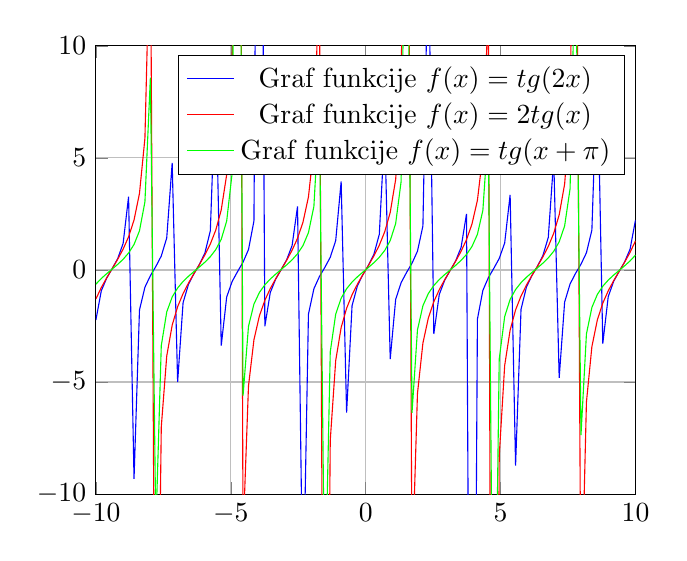
\begin{tikzpicture}
            \begin{axis}[
                grid=major,
                ymin=-10,
                ymax=10,
                xmin=-10,
                xmax=10,
            ]
                \addplot[
                    color = blue,
                    samples = 100,
                    domain = -10:10
                ]{tan(deg(2*x))};
                \addlegendentry{Graf funkcije  \(f(x) = tg(2x)\)}
                \addplot[
                    color = red,
                    samples = 100,
                    domain = -10:10
                ]{2*tan(deg(x))};
                \addlegendentry{Graf funkcije  \(f(x) = 2tg(x)\)}
                \addplot[
                    color = green,
                    samples = 100,
                    domain = -10:10
                ]{tan(deg(x + 3.1515))};
                \addlegendentry{Graf funkcije  \(f(x) = tg(x + \pi)\)}
            \end{axis}
        \end{tikzpicture}
        \caption{Grafovi funkcija tangens i kotangens s raznim parametrima}
        \label{fig:template}
    \end{figure}
    \\
   
\subsubsection{Nultočke i točke u kojima graf sječe y-os \trig}
    Pošto su trigonometrijske funkcije periodične imaju mnogo nultočaka.
    Funkcija kosunus ima dvije nultočke na svakom periodu:
    \begin{equation*}
        \begin{split}
            sin(x) &= 0 \\
            x &= k\pi,\; k \in \mathbb{Z} 
        \end{split}
    \end{equation*}
    Funkcija tangens ima nultočku na svakom periodu.
    \begin{equation*}
        \begin{split}
            tg(x) &= 0 \\
            x &= \frac{\pi}{2},\; k \in \mathbb{Z} 
        \end{split}
    \end{equation*}

\subsubsection{Parnost i neparnost \trig}
    Sinus je neparna funkcija, kosinus parna, tangens parna, a kotanges neparna.

\subsubsection{Periodičnost \trig}
    Sve trigonometrijske funkcije su periodične. Za sve vrijedi:
    \[f(x + P) = f(x), P \neq 0\]
    Temeljni period funkcije sinus je \(2\pi\), a funkcije tanges je \(\pi\).

\subsubsection{Monotonost \trig}
    Trigonometrijske funkcije su monotone samo na određenim intervalima.
    
\subsubsection{Omeđenost \trig}
    Funkcija sinus je omeđena odozdo i odozgo s \(\abs{1}\). Funkcije tanges i kotangens nisu omeđene.

\subsubsection{Injektivnost i surjektivnost \trig}
    Trigonometrijske funkcije su surjekcije jer su periodične. 

\subsubsection{Inverz \trig}
    Trigonometrijske funkcije imaju inverze samo na intervalima od nula uključivo do njihovog temeljnog perioda.